\subsection{Two-Container}
\subsubsection{Two-Container CPU Utilization}
\begin{itemize}
    \item CPU utilization in the two-container configuration may vary depending on the distribution of workload between the containers.
    \item Both containers can handle requests, potentially balancing the load and leading to lower overall CPU utilization.
    \item Under peak demand, CPU usage may increase as both containers manage incoming requests simultaneously.
\end{itemize}

\noindent Below is the graph that illustrates the CPU utilization for two-container configuration:

\begin{figure}[h]
    \begin{minipage}[t]{0.5\textwidth}
        \centering
        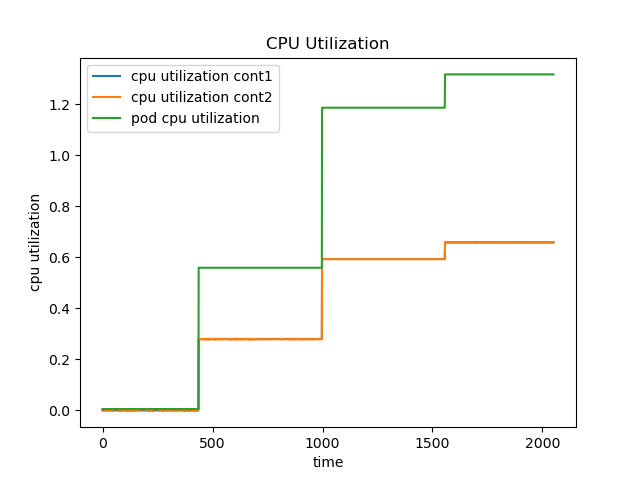
\includegraphics[width=0.9\textwidth]{../sample_results/loop/two-container/cpu-utilization-two-container.png}
        \caption{Loop}
    \end{minipage}
    \hfill
    \begin{minipage}[t]{0.5\textwidth}
        \centering
        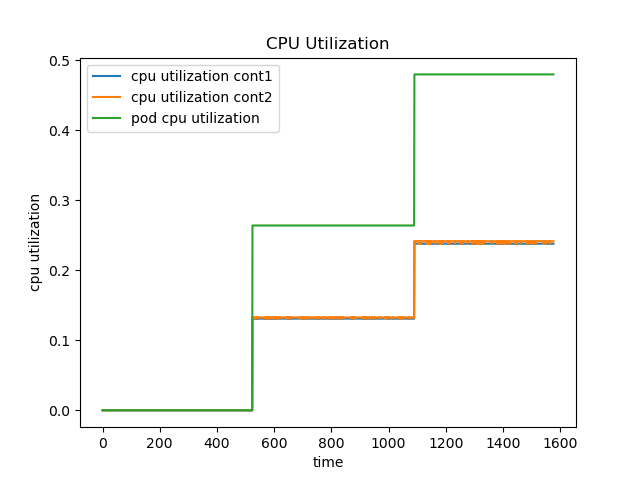
\includegraphics[width=0.9\textwidth]{../sample_results/lorem/two-container/cpu-utilization-two-container.png}
        \caption{Lorem}
    \end{minipage}
\end{figure}

\newpage
\subsubsection{Two-Container Response Time Observations}
\begin{itemize}
    \item Response times in the two-container configuration can be lower, as multiple containers share the workload.
    \item If one container becomes overwhelmed, the other can handle the load, potentially balancing response times.
    \item During peak demand, response times may fluctuate depending on the distribution of requests between the containers.
\end{itemize}

\noindent Below are the response time graphs for two-container configuration:

\begin{figure}[h]
    \begin{minipage}[t]{0.5\textwidth}
        \centering
        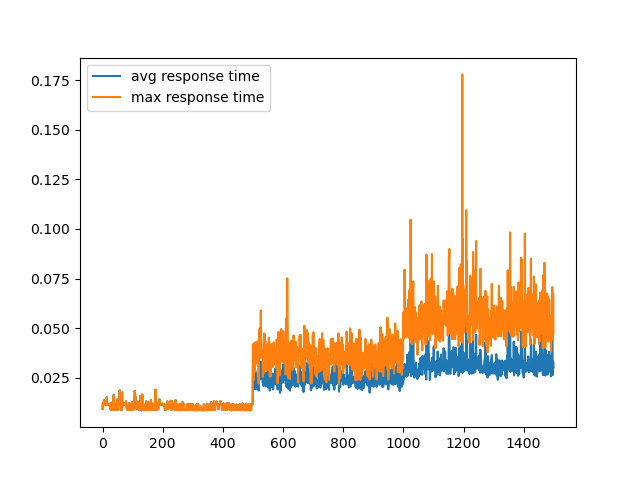
\includegraphics[width=0.9\textwidth]{../sample_results/loop/two-container/response-time-two-container-two-container.png}
        \caption{Loop}
    \end{minipage}
    \hfill
    \begin{minipage}[t]{0.5\textwidth}
        \centering
        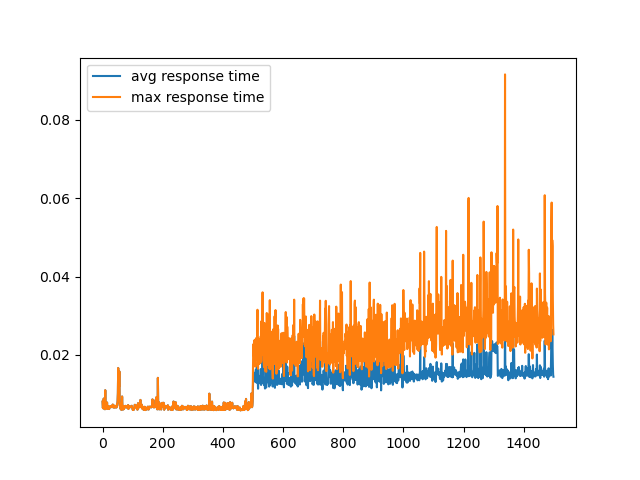
\includegraphics[width=0.9\textwidth]{../sample_results/lorem/two-container/response-time-two-container-two-container.png}
        \caption{Lorem}
    \end{minipage}
\end{figure}

\newpage
\subsubsection{Two-Container Memory Utilization}
\begin{figure}[h]
    \begin{minipage}[t]{0.5\textwidth}
        \centering
        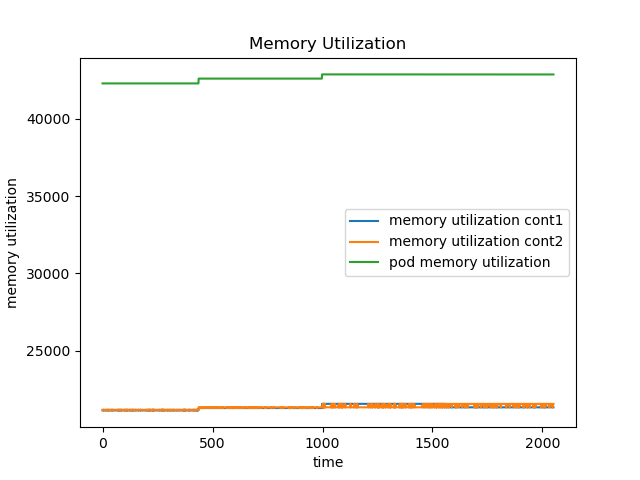
\includegraphics[width=0.9\textwidth]{../sample_results/loop/two-container/mem-utilization-two-container.png}
        \caption{Loop}
    \end{minipage}
    \hfill
    \begin{minipage}[t]{0.5\textwidth}
        \centering
        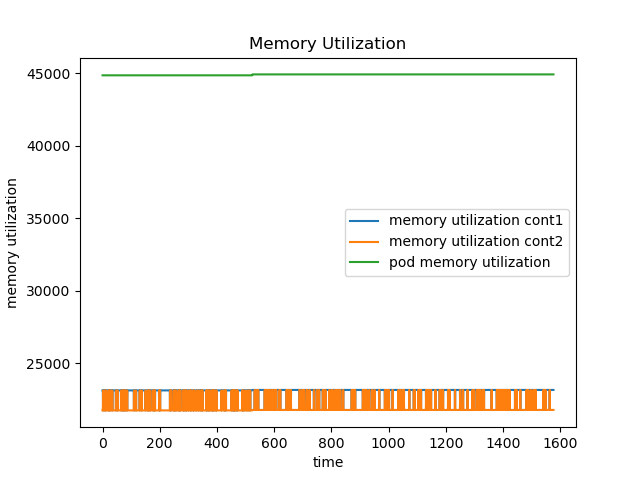
\includegraphics[width=0.9\textwidth]{../sample_results/lorem/two-container/mem-utilization-two-container.png}
        \caption{Lorem}
    \end{minipage}
\end{figure}

\begin{itemize}
    \item Memory utilization in the two-container configuration can vary depending on the memory demands of the workloads.
    \item Each container manages its own memory allocation, which may lead to more efficient usage when workloads are balanced.
    \item As workloads stabilize, memory utilization should even out as both containers manage their respective resources.
\end{itemize}

